%  LaTeX support: latex@mdpi.com
%  In case you need support, please attach all files that are necessary for compiling as well as the log file, and specify the details of your LaTeX setup (which operating system and LaTeX version / tools you are using).

% You need to save the "mdpi.cls" and "mdpi.bst" files into the same folder as this template file.

%=================================================================
\documentclass[sustainability,article,submit,moreauthors,pdftex,10pt,a4paper]{mdpi} 

%--------------------
% Class Options:
%--------------------
% journal
%----------
% Choose between the following MDPI journals:
% actuators, admsci, aerospace, agriculture, agronomy, algorithms, animals, antibiotics, antibodies, antioxidants, applsci, arts, atmosphere, atoms, axioms, batteries, behavsci, beverages, bioengineering, biology, biomedicines, biomimetics, biomolecules, biosensors, brainsci, buildings, carbon, cancers, catalysts, cells, challenges, chemosensors, children, chromatography, climate, coatings, computation, computers, condensedmatter, cosmetics, cryptography, crystals, data, dentistry, designs, diagnostics, diseases, diversity, econometrics, economies, education, electronics, energies, entropy, environments, epigenomes, fermentation, fibers, fishes, fluids, foods, forests, futureinternet, galaxies, games, gels, genealogy, genes, geosciences, geriatrics, healthcare, horticulturae, humanities, hydrology, informatics, information, infrastructures, inorganics, insects, instruments, ijerph, ijfs, ijms, ijgi, inventions, jcdd, jcm, jdb, jfb, jfmk, jimaging, jof, jintelligence, jlpea, jmse, jpm, jrfm, jsan, land, languages, laws, life, literature, lubricants, machines, magnetochemistry, marinedrugs, materials, mathematics, mca, mti, medsci, medicines, membranes, metabolites, metals, microarrays, micromachines, microorganisms, minerals, molbank, molecules, mps, nanomaterials, ncrna, neonatalscreening, nutrients, particles, pathogens, pharmaceuticals, pharmaceutics, pharmacy, philosophies, photonics, plants, polymers, processes, proteomes, publications, recycling, religions, remotesensing, resources, risks, robotics, safety, sensors, separations, sexes, sinusitis, socsci, societies, soils, sports, standards, sustainability, symmetry, systems, technologies, toxics, toxins, universe, urbansci, vaccines, vetsci, viruses, water
%---------
% article
%---------
% The default type of manuscript is article, but can be replaced by: 
% addendum, article, book, bookreview, briefreport, casereport, changes, comment, commentary, communication, conceptpaper, correction, conferencereport, expressionofconcern, meetingreport, creative, datadescriptor, discussion, editorial, essay, erratum, hypothesis, interestingimage, letter, newbookreceived, opinion, obituary, projectreport, reply, retraction, review, sciprints, shortnote, supfile, technicalnote
% supfile = supplementary materials
%----------
% submit
%----------
% The class option "submit" will be changed to "accept" by the Editorial Office when the paper is accepted. This will only make changes to the frontpage (e.g. the logo of the journal will get visible), the headings, and the copyright information. Also, line numbering will be removed. Journal info and pagination for accepted papers will also be assigned by the Editorial Office.
%------------------
% moreauthors
%------------------
% If there is only one author the class option oneauthor should be used. Otherwise use the class option moreauthors.
%---------
% pdftex
%---------
% The option pdftex is for use with pdfLaTeX. If eps figure are used, remove the option pdftex and use LaTeX and dvi2pdf.

%=================================================================
\firstpage{1} 
\makeatletter 
\setcounter{page}{\@firstpage} 
\makeatother 
\articlenumber{x}
\doinum{10.3390/------}
\pubvolume{xx}
\pubyear{2016}
\copyrightyear{2016}
\externaleditor{Academic Editor: name}
\history{Received: date; Accepted: date; Published: date}
%------------------------------------------------------------------
% The following line should be uncommented if the LaTeX file is uploaded to arXiv.org
%\pdfoutput=1

%=================================================================
% Add packages and commands here. The following packages are loaded in our class file: fontenc, calc, indentfirst, fancyhdr, graphicx, lastpage, ifthen, lineno, float, amsmath, setspace, enumitem, mathpazo, booktabs, titlesec, etoolbox, amsthm, hyphenat, natbib, hyperref, footmisc, geometry, caption, url, mdframed

%=================================================================
%% Please use the following mathematics environments:
 \theoremstyle{mdpi}
 \newcounter{thm}
 \setcounter{thm}{0}
 \newcounter{ex}
 \setcounter{ex}{0}
 \newcounter{re}
 \setcounter{re}{0}

 \newtheorem{Theorem}[thm]{Theorem}
 \newtheorem{Lemma}[thm]{Lemma}
 \newtheorem{Corollary}[thm]{Corollary}
 \newtheorem{Proposition}[thm]{Proposition}

 \theoremstyle{mdpidefinition}
 \newtheorem{Characterization}[thm]{Characterization}
 \newtheorem{Property}[thm]{Property}
 \newtheorem{Problem}[thm]{Problem}
 \newtheorem{Example}[ex]{Example}
 \newtheorem{ExamplesandDefinitions}[ex]{Examples and Definitions}
 \newtheorem{Remark}[re]{Remark}
 \newtheorem{Definition}[thm]{Definition}
%% For proofs, please use the proof environment (the amsthm package is loaded by the MDPI class).

%=================================================================
% Full title of the paper (Capitalized)
\Title{Title}

% Authors, for the paper (add full first names)
\Author{Caroline Jennings Saul $^{1, 2}$ and Heiko Gebauer $^{1,2}$}
% Authors, for metadata in PDF
\AuthorNames{Caroline Jennings Saul, Heiko Gebauer}

% Affiliations / Addresses (Add [1] after \address if there is only one affiliation.)
\address{%
$^{1}$ \quad Eawag: Swiss Federal Institute of Aquatic Science and Technology, Environmental Social Sciences, Überlandstrasse 133, 8600 Dübendorf, Switzerland;\\
$^{2}$ \quad Affiliation 2; e-mail@e-mail.com}

% Contact information of the corresponding author
\corres{Correspondence: caroline.saul@eawag.ch; Tel.: +41 58 765 5441}

% Current address and/or shared authorship
%\firstnote{Current address: Überlandstrasse 133, P.O. Box, 8600 Dübendorf, Switzerland} 
%\secondnote{These authors contributed equally to this work.}

% Simple summary
%\simplesumm{}

% Abstract (Do not use inserted blank lines, i.e. \\) 
\abstract{A single paragraph of about 200 words maximum. For research articles, abstracts should give a pertinent overview of the work. We strongly encourage authors to use the following style of structured abstracts, but without headings: 1) Background: Place the question addressed in a broad context and highlight the purpose of the study; 2) Methods: Describe briefly the main methods or treatments applied; 3) Results: Summarize the article's main findings; and 4) Conclusion: Indicate the main conclusions or interpretations. The abstract should be an objective representation of the article: it must not contain results which are not presented and substantiated in the main text and should not exaggerate the main conclusions.}

% Keywords List three to ten pertinent keywords specific to the article, yet reasonably common within the subject discipline.
\keyword{keyword 1; Container Based Sanitation; IoT; service innovation; BoP }

% The fields PACS, MSC, and JEL may be left empty or commented out if not applicable
%\PACS{J0101}
%\MSC{}
%\JEL{}

% If this is an expanded version of a conference paper, please cite it here: enter the full citation of your conference paper, and add $^\S$ in the end of the title of this article.
%\conference{}

%%%%%%%%%%%%%%%%%%%%%%%%%%%%%%%%%%%%%%%%%%
% Only for the journal Data:

%\dataset{DOI number or link to the deposited data set in cases where the data set is published or set to be published separately. If the data set is submitted and will be published as a supplement to this paper in the journal Data, this field will be filled by the editors of the journal. In this case, please make sure to submit the data set as a supplement when entering your manuscript into our manuscript editorial system.}

%\datasetlicense{license under which the data set is made available (CC0, CC-BY, CC-BY-SA, CC-BY-NC, etc.)}

%%%%%%%%%%%%%%%%%%%%%%%%%%%%%%%%%%%%%%%%%%
\begin{document}

%%%%%%%%%%%%%%%%%%%%%%%%%%%%%%%%%%%%%%%%%%
%% Sections that are not mandatory are listed as such. The section titles given are for Articles. Review papers and other article types have a more flexible structure. 

%% Only for the journal Gels: Please place the Experimental Section after the Conclusions

%%%%%%%%%%%%%%%%%%%%%%%%%%%%%%%%%%%%%%%%%%
%\setcounter{section}{-1} %% Remove this when starting to work on the template.
%\section{How to Use this Template}

%The template details the sections that can be used in a manuscript. Sections that are not mandatory are listed as such. The section titles given are for Articles. Review papers and other article types have a more flexible structure. For any questions, please contact the editorial office of the journal or support@mdpi.com. For LaTeX related questions please contact Janine Daum at latex-support@mdpi.com.

\section{Introduction}



Digital technologies are playing a growing role in the extension of energy, finance/retail \cite{Berger2013}, health, media, educational, and water \cite{Gebauer2014} services to Base of the Pyramid (BoP) populations, and the sanitation sector also stands to benefit. This paper looks at the role of digitalization in organizations that offer Container Based Sanitation (CBS) services. CBS provides an opportunity not only to offer a dignified sanitation solution to some of the 2.3 Billion people who do not have access to basic sanitation and increase the proportion of population whose excreta is safely managed, which is currently at 39 percent \cite{WHO2017}, but to capture and harness relatively undiluted product/waste/excreta streams for conversion into  useful resources. 

.

Systems that resemble CBS technically have been seen in the past, and have either been replaced with water-born sanitation [EXAMPLES] or have been abandoned due to [.....]. The a holistic Product-service-system approach (and innovations thereof) taken by these "new" CBS service providers will determine if this actually represents one of the novel approaches to excreta management that is necessitated by changes in demographics, resource availability (climate), 

.

Can the digitalization of these service models enable their survival? 
.

Additionally, new excreta management solutions are needed in the face of rapid urbanization, less water.... \cite{Larsen2016}

. 

This Design section of this article discusses that appropriateness and application of the case study methodology. The Context sections discusses the basic Product-Service System (PSS) of CBS, some historical challenges similar systems have encountered (or sources of failure), the relationship between CBS and the circular economy and other examples of digitalization for the provision of services in low-income countries. The Results and Discussion section (    ) the findings of the cross-case analysis and () considers future directions for (). 


%%%%%%%%%%%%%%%%%%%%%%%%%%%

\section{Design and Methodology}

There are fewer than ten(?) (private?) organization offering container based sanitation services, so a purposeful sampling approach was taken, selecting organizations that exhibited particularly distinctive or swift approaches to incorporating digital technologies into their operations.

The organizations service between 100 and 1000(?) toilets, providing safely managed sanitation for  XXX, and have staffs ranging from XX to XXX. Two of the organizations operate in Africa and one in South America. 

The method relies on a longitudinal case study approach. The development and growth of these  organizations has been followed over the course of three to five years through workshops, site visits, and an ongoing series of interviews, including one semi-structured specifically about the role of digital technologies in their operations. Secondary data including publications from the organizations and third parties has also been included for triangulation purposes. 

Instances of digitalization exhibited by each organization were illustrated using XXXXX's technological stack framework and the influence of each of these applications of digitalization on the business model of each organization has been considered. For the purposes of this analysis digitalization includes a wide variety of activities, ranging from transitioning paper-based records to a computer database to incorporating the Internet of Things into their service delivery model. 

%The examples/evidence of digitalization in these organizations was plotted into 
%illustrated the "tech stacks"of each of the organizations using XXXX's layered architecture framework.
%At it's core, CBS services and most other safely managed sanitation services will involve the movement of physical products, so "digital services" was modified to simply "services" and as not all aspects of digitalization are IoT based (transitioning from paperbased record keeping to using excel or a database are also valid examples) "Sensor and Actuator" is phased as "inputs or data source" 



%%%%%%%%%%%%%%%%%%%%%%%%%%%%%%%%%%%%%%%%%%


\section{Context}
In 2015 the United Nations passed 17 Sustainable Development Goals, which include Goal 6.2: "By 2030, achieve access to adequate and equitable sanitation and hygiene for all and end
open defecation, paying special attention to the needs of women and girls and those in vulnerable
situations" and 6.3: "By 2030, improve water quality by reducing pollution, eliminating dumping and minimizing release of hazardous chemicals and materials, halving the proportion of untreated wastewater and substantially increasing recycling and safe reuse globally" \cite{UNICEF2015}.

892 million people practice open defecation, but the excreta of an additional 3.5 billion people who have access to shared or basic sanitation is not safely managed, i.e. treated \cite{WHO2017}. Safely managed sanitation requires consideration beyond the toilet – the whole sanitation chain must be considered. This includes how and where excreta enters a sanitation system; how and for how long it is contained on site; how it is transported to a treatment facility, if it is not treated on-site; how it is treated; and how it is finally disposed of or re-utilized \cite{Tilley2014}. The necessary products and services for all of these activities to be carried out can be offered by a single or multiple organizations. The successful delivery of such services is complex given the personal nature of the services and the public health risks posed by an accident.  
% * <saulcj@gmail.com> 2017-11-07T08:43:20.374Z:
%
% >  public health risks posed by an accident
%
% ^.

%Sanitation in general, SDGS, shame, OD, gaps in services/safe management, needs leap in customer value, to deliver complex services

Management and digital technologies play a vital role in making the leap to deliver complex services. 
\subsection{Container Based Sanitation}

Container based sanitation (CBS) refers to a sanitation system in which excreta is stored in a sealable vessel at the point of use and later transported to a treatment site with pushcarts or motorized vehicles, where it is safely handled and treated. Organizations are implementing these systems in areas densely populated urban and peri-urban areas where conventional sanitation technologies, such as sewers and on-site sanitation solutions, like septic tanks and improved pit latrines, are not realistic or feasible due to political, geographic, or financial forces. Many organizations harness the nutrient and energy resources that are contained in the excreta. 


 
\subsubsection{History}

Similar "removal" style sanitation systems have been put into place throughout history in, for example, the United Kingdom (cite), Australia (cite), Japan (cite), Kenya  (cite), Bolivia (cite) and South Africa (cite). These systems have largely been replaced with on-site or waterborne sanitation and have been regarded as problematic financially, socially, and with regard to human rights. 

For example, residents of a South African township that is still served by a so called "bucket system" protested after their loos had not been serviced for (   ). (cite)

world war ii prevented the importation of buckets

expensive and becoming obsolete, Bloomfield1947 in \cite{Nyanchaga2007}

Need constant supervision through the collection process Russell1957 in \cite{Nyanchaga2007}

bad roads, 



in rapidly urbanizing areas the building of sewers and treatment capacity has not kept pace with population growth 


concerns about shared facilities




\subsubsection{Current state}

Starting in the early 2000s, these CBS systems have been implemented as household subscription services, public toilets, and franchisee businesses in Africa, Latin America, and the Caribbean. These service providers market their service to households and in some cases entrepreneurs. Once someone decides to use the service, they sign a contract and begin renting a toilet. Most of the toilet designs separate the urine from the feces; in this case, after a bowel movement the user adds ash, sawdust, bagasse, peanut shells, or another locally available cover material to help control odor. When the toilet is used, the excreta is stored in containers; depending on the design, containers include a mix of jugs, barrels, bags, buckets, and films. The cartridges are regularly collected, some organizations only collect the feces cartridges. When the customer is a household, collection is generally once or twice a week, but for larger producers, like franchisees it can be daily. Service providers must collect payments from customers and occasionally repair toilets or make emergency collections of excreta or deliveries of cover material. The excreta is transported to a treatment or disposal site. Depending on the organization and type of excreta, this could mean combination of disposal or resource recovery options including: depositing it at a municipal wastewater treatment or fecal sludge management plant, composting, anaerobic digestion, processing into protein or fertilizer, and solar hygeinization. 


In a seventeen week field trail with a household CBS service, participants almost totally ceased open defecation, although some use of pit-latrines and public toilets remained \cite{Tilmans2015}. At the end of this same pilot, participants reported being less ashamed and feeling safer, more modern, and prouder of their sanitation situation than their neighbors in both their informal settlement and an adjacent formal settlement\cite{Russel2015}.

%One organization rents their toilet and superstructures to entrepreneurs in a franchise model
% * <saulcj@gmail.com> 2017-10-19T10:20:54.171Z:
% 
% > and franchisee businesses
% trying to think of a better way to describe what sanergy does, since someof them are for private business use (zB if a bar rents one)
% 
% ^.



%household, free public, public franchise


%"pride, modernity and safety (all p<0.001). S/he was also significantly less likely to report feeling ashamed of" 



 
 source separation and undilution
 
(user acceptance of)


why an advanced service
- quality demand
- low income of consumers/selling difficult
- low economies of scale
-  complex collection

In these types of systems, customer destiny, \cite{Schmitt2017}

In contrast to the "bucket systems" of the past, these service providers 

They face many of the same challenges as these former system operators do, such as the as difficult terrain, poor roads, dispersed collection points and time-sensitive nature of collection mentioned by ProvencialMedicalOfficer1952 in \cite{Nyanchaga2007}; however, as their customers are actual customers (and not citizens receiving a govt provided service), they face pressures to () as there are other alternatives, such as shared or public latrines, open defecation, or (). %". In this setting, it appears that well-designed toilets and professionalized collection service procedures can also avoid the stigma historically associated with bucket latrines and similar “low-tech” options" \cite{Russel2015}


\subsubsection{Resource Recovery}

Conventional wastewater (blackwater) contains  water, energy and material resources \cite{Guest2009}. Depending on the desired utilization of these resources, collecting residuals in the purest possible form, i.e., undiluted by flushing water, reduces the effort and additional inputs needed to process them later. This is extended further when source separation methods are used, containing, collecting, storing, conveying, and treating urine separately from fecal matter. This has the added benefit for the user of reducing odor in the toilet (CITE). In order for the effort put into extracting energy and materials from the products collected through CBS services to be worthwhile/impactful/attractive products need to be collected swiftly and in sufficient volume. When writing about more generalized source separated or decentralized systems, \cite{Tilley2013} calls for "more affordable and efficient conveyance technologies are needed to support the decentralized transfer of products between producers and consumers"

The different approaches to resource recovery taken by the organizations in this analysis can be seen in Table.



\subsubsection*{Water}
Since most CBS systems are waterless, we primarily are concerned with the energy and material resources contained in excreta. The lack of conventional use of water for flushing and conveyance is in itself interesting when considering the impact of such systems on the environment and their adaptability to various contexts; however it is outside the scope of this analysis. although, the lack of additional water can be seen as a bonus in these systems for collecting undiluted products, as (in contrevention of) conventional sewers, there is no provision for the collection and disposal of greywater that is generated on premises. \cite{Tilmans2015} 

\subsubsection*{Energy}
CBS service providers are regard the excrement that they collect as an energy carrier and harness this energy via anaerobic digestion, a process by which organic matter is xxxx, resulting in a gas that is a mixture of methane, carbon dioxide and xxxx.  

excretia is also fed to Black Soldier fly larvae, which are harvested and can be used as inputs to animal feed or have oil extracted from them. 

binder in briquettes



\subsubsection*{Material}
Applying excrement to agricultural land or even burning it is nothing new, it goes back centuries, but these systems have often lacked accountability and hygiene. (direct land application, dumping into water-bodies…). Additionally, some farmers are no longer interested because cheap chemical fertilizers are avoidable and the transport costs were not worth it.

Material: nutrients (NPK in urine), soil amendment from composted or vermicomposted excreta, feces as a food for bsf
 
  CBS services provide for relatively frequent collection of excreta (daily, biweekly, and weekly) , which provides 
  
  The characteristics of urine change over time based on the @kai

\subsection{Digitalization of services in the Global South}

Mobile money (Mpesa - Heiko do you have some sources from HSG?)
smart metering (solar home systems)
apps reinventing (safe boda)
mHealth stuff?

%%%%%%%%%%%%%%%%%%%%%%%%%%%%%%%%%%%%%%%%%%
\section{Results}
The CBS service providers that were considered in this analysis cover the entire sanitation chain, from user interface to reuse or disposal, but have different approaches to  ensuring , as seen in Table \ref{tbl:SanChain}

\begin{table}[H]
\caption{Most container based sanitation service providers account for the entire sanitation chain}
\label{tbl:SanChain}
\small % Font size can be changed to match table content. Recommend 10 pt.
\centering
\begin{tabular}{ p{.09\textwidth} |p{.15\textwidth} p{.15\textwidth} p{.15\textwidth} p{.15\textwidth} p{.15\textwidth} }
\toprule
& \textbf{User Interface} & \textbf{Containment}	 & \textbf{Conveyance} &\textbf{Treatment} &\textbf{Reuse or Disposal}\\
\midrule
xRunner		
& Urine diverting dry toilet
	& Excreta barrels are lined with a plastic bag
  & Collected once a week by truck 
  & Composting 
  & Compost used by gardeners and landscapers\\
Sanivation 
& UDDT (?)
& Excreta barrels are lined with a plastic bag
& Bags are collected by tuktuk twice a week. 
& Solar hygenization
& Hygenized fecal sludge is mixed with chardust to for briquettes for cooking and heating\\
LooWatt		
& Different models of dry toilets, some urine diverting, excreta is sealed in plastic film by the user

& Excreta are sealed into plastic film via a flushing motion by the user. This sealed material sits in a barrel.

& Barrels are collected once a week by a push cart
	 
&  Anaerobic digestion, pasteurization

& Biogas used in CHP generator \newline Pasteurized digestate used by farmers, some digestate mixed with rice husks for vermicomposting\\
%Sanergy  & & \\
%SOIL &s & & Mobile Money (forthcoming pilot)\\
\bottomrule
\end{tabular}
\end{table}

\subsection{Applications of Digital Technologies}
The organizations considered in this analysis demonstrate 

The digital architectures for each of the organizations center around their Customer Relationship Management platforms, but the way data enter these platforms varies from organization to organization, as seen in Table \ref{tbl:digFramework}.




\begin{table}[H]
\centering
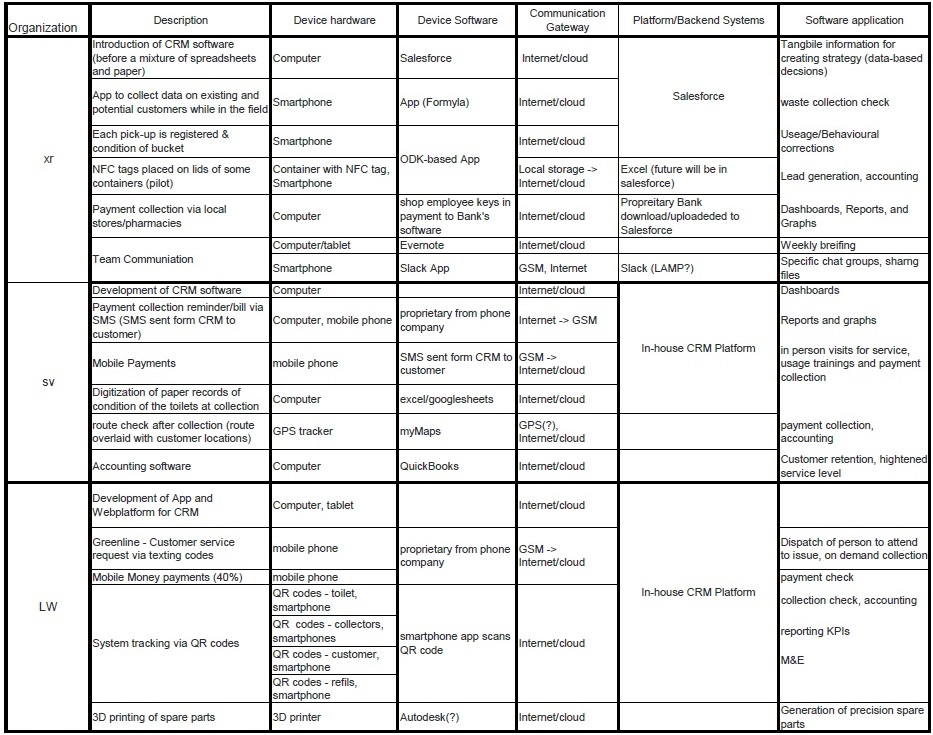
\includegraphics[width=\textwidth]{digFramTbl.jpg}
\caption{This table shows the digital technological stacks of each of the organizations. (will be transfered to LATEX, but want to check the contents first)}
\label{tbl:digFramework}
\end{table}   

The introduction of technologies are primarily observed to address three categories of obstacles the organizations have faced: logistics, payments and information management. 

\begin{table}[H]
\caption{This is a table caption. Tables should be placed in the main text near to the first time they are cited.}
\label{tbl:BMfx}
\small % Font size can be changed to match table content. Recommend 10 pt.
\centering
\begin{tabular}{ p{.09\textwidth} |p{.26\textwidth} p{.26\textwidth} p{.26\textwidth} }
\toprule
& \textbf{Logistics} & \textbf{CRM}	 & \textbf{Payments}\\
\midrule
xRunner		& NFC Tags + ODK App	& Salesforce + Formyoula App  & interbank in-shop payments\\
Sanivation & GPS route recorder & Own database + SMS & mPesa (Mobile moeny) + QuickBooks \\
LooWatt		& QR-codes + 3D printer & Web Platform + Greenline	 &  Mobile Money \\
%Sanergy  & & \\
%SOIL &s & & Mobile Money (forthcoming pilot)\\
\bottomrule
\end{tabular}
\end{table}

\subsection{Development}
off the shelf

developers from the "North"

local development

Most organizations started recordkeeping using a mishmash of spreadsheets and paper and have followed different strategies to make more sophisticated systems that address their specific needs. %from sandec

x-runner and LooWatt worked with international developers to build their software systems. They received external grants to fund the process. In both cases, the organizations worked with their developers over about half a year, using tools like Skype to design the process flows. Then the developers visited the locations in order to tweak the software and train the organizations on how to use them. Sanivation’s CRM system was built by a Kenyan developer over three months and financed out of internal funds. %from sandec

It is important for organizations to understand what is possible for tech to accomplish and for developers to understand the context for which they are designing. %from sandec

The limited network coverage means that the apps need to work offline, which means that generally, the applications use quite a bit of memory, considering   the quality of  smartphones that the organizations have access to. %from sandec

For LooWatt it was important to design an app that could be used by collectors with limited literacy. It has also been difficult for people to use the app while wearing personal protection equipment during collection.  %from sandec



\subsubsection{Logistics}
All three organizations have applied different digital tools to improve their logistics. x-runner and LooWatt have incorporated the Internet of Things into physical aspects of their systems for tracking interactions. x-runner has outfitted the lids of about half of their barrels with near-field communication (NFC) tags. At collection, these lids are scanned with an application built with Open Data Kit (ODK), which also verifies that the customer has paid their monthly bill and allows the collector to make notes about the condition of the barrel.  LooWatt has QR-codes on their Barrels, refills, toilets, etc. At collection, the toilet and bucket QR codes are scanned and the weight of the barrel is entered into the App. Once they arrive at the treatment site, the barrels are scanned and weighed again, providing a layer of accountability that the excreta actually makes it to the treatment site. 

Sanivation's collectors carry a GPS logger with them, so at the end of each day, the route taken can be overlaid onto a map of the customers who should have been served to check that each household has been serviced.

In response to the bottlenecks and expense of importing individual replacement parts, LooWatt uses a 3D printer, which can produce components that exceed the quality and precision of those constructed out of local materials. 





\subsubsection{Payments}
Collecting rental/subscription fees from households has been a pain point for many CBS organizations. It is time and labor intensive: money collectors faced security risks, received incomplete payments, skimmed off the top, and sometimes found it difficult to track-down customers. To address this, organizations have looked to electronic payment methods. x-Runner's customers pay for their sanitation service in at stores and pharmacies through a service from Banco de Crédito del Perú. The customer pays a clerk, who inputs the transaction into a computer. Later, x-runner can download the payment data from the bank and upload it into their CRM system. 

LooWatt and Sanivation are introducing mobile money payments. 
"We just limit the ways we accept cash"
Sanivation can send payment reminders and promotions directly to their customers' cellphones from their CRM system.
 Both organizations have found that they have had to work with customers individually to get them aquainted with using these platforms. 


\subsubsection{Customer Relationship Management}
Each organization has developed an internal database for keeping track of the interactions that they have with customers. 

These databases 

Starting from when a customer first voices an interest in having a toilet installed, x-runner enters their information into an application called Formyoula and their customer profile is created. This app works offline, which is important in areas with spotty cellphone coverage, and is synced daily with Salesforce, a customer relationship management (CRM) system. Once they have a profile, the sales team can visit their home and sign a contract. This initial survey forms the basis of the customer’s database entry where their service history and other behavioral data are stored.%from sandec

Sanivation’s bespoke CRM system provides a structure to keep track of customer data such as household size and wealth, payment history, amount of excreta generated, as well as their referral history and account manager.  Most of their operations data collection, like bucket weight and condition, is done by pen and paper – taken down by hand and keyed in to the system later.%from sandec

LooWatt uses a web-platform to house their database that stores all of the QR scans and payment history.  This aggregates cash and mobile money payments and allows managers to see if customers still have credit to access refills and services. Additionally, their customers can contact them using a free SMS system to request technical service, additional refills, or an on-demand collection. These appeals are registered in their web-platform and the manager can send someone to attend to the request. %from sandec

Each of these systems is different, but theorgnizations enjoy that their  new systems keep all the information in one place and easier to collect. With real-time data on hand, of users can easily create clear graphs and charts for meetings and reports. This can  guide  decision-making processes.. %from sandec







\subsection{Challenges and Opportunities}
Future 
(blockchain?)

Data that is collected now, will be useful in developing future strategies. 

Notably, none of these organizations are currently using digital routing to optimize collection; although it s something they are interested in in the future. 

Everyone is anticipating the next version of their systems, now that they better understand the gaps, issues, and potential of their software.  Inspiration is being drawn from providers of other basic services, such as household solar pay-as- you-go, and from other sanitation and logistics businesses. %from sandec

LooWatt notes that their app isn’t really needed to manage their day to day operations with just 100 toilets, but if they want to scale they need to understand the behavior of their customers. This is much easier to do when the data is digital. Additionally, the app and web-platform standardizes the quality assurance of their system and creates a template for replication and future franchising opportunities. %from sandec

Sanivation’s toilet service representatives carry a GPS tracker; their path from each day is downloaded and overlaid on a map of their customers, to act as a check that all households were served. As companies grow, this could be taken a step further, by using route optimizing software; however, in many cases better maps of roads and pathways would be needed. 
CBS service providers are innovating independently to craft IT systems that fit their specific needs, context, and growth plans. These systems have been able to unlock new potential in the organizations’ business models. CBS organizations are exchanging experiences with each other to strengthen their systems and may collaborate more formally in the future. %from sandec


%%%%%%%%%%%%%%%%%%%%%%%%%%%%%%%%%%%%%%%%%%
\section{Discussion}
Different approaches to solving similar obstacles 

Introducing digital tools requires 


\subsection{Role in Business Model Innovation}


\begin{figure}[H]
\centering
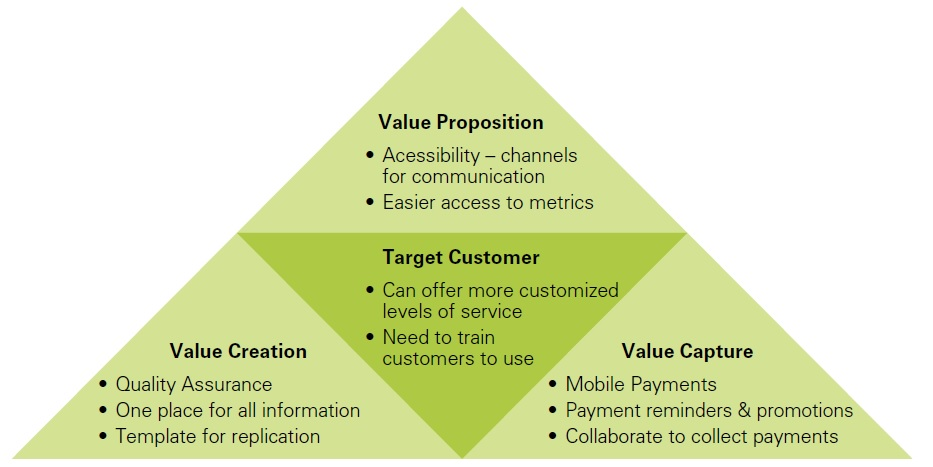
\includegraphics[width=\textwidth]{bmt.jpg}
\caption{This business model triangle shows the areas of a CBS business models where digitalization has h (will be transfered to LATEX, but want to check the contents first)}
\label{fig:bmt}
\end{figure}  

CBS organizations cannot contribute to the circular economy if they cannot first fulfill their value proposition to the users of their toilets and they can have a larger impact on closing resource loops, the more excreta they collect.  

%%%%%%%%%%%%%%%%%%%%%%%%%%%%%%%%%%%%%%%%%%
\section{Conclusions}

This section is not mandatory, but can be added to the manuscript if the discussion is unusually long or complex.

%%%%%%%%%%%%%%%%%%%%%%%%%%%%%%%%%%%%%%%%%%
\vspace{6pt} 

%%%%%%%%%%%%%%%%%%%%%%%%%%%%%%%%%%%%%%%%%%
%% optional
\supplementary{The following are available online at www.mdpi.com/link, Figure S1: title, Table S1: title, Video S1: title.}

%%%%%%%%%%%%%%%%%%%%%%%%%%%%%%%%%%%%%%%%%%
\acknowledgments{
Resources for conducting these cases were received from SDC and the eawag discretionary fund. LIB4RI covered the costs for open access publishing. }
% * <saulcj@gmail.com> 2017-10-19T09:28:43.954Z:
% 
% > ndicate grants
% was this supported by any grants? just the SDC one?
% 
% ^ <saulcj@gmail.com> 2017-10-19T09:29:08.735Z.
% * <saulcj@gmail.com> 2017-10-19T09:28:19.476Z:
% 
% > funds for covering the costs to publish in open acce
% is this Lib4Ri?
% 
% ^ <saulcj@gmail.com> 2017-10-19T09:28:35.027Z.

%%%%%%%%%%%%%%%%%%%%%%%%%%%%%%%%%%%%%%%%%%
%\authorcontributions{For research articles with several authors, a short paragraph specifying their individual contributions must be provided. The following statements should be used ``X.X. and Y.Y. conceived and designed the experiments; X.X. performed the experiments; X.X. and Y.Y. analyzed the data; W.W. contributed reagents/materials/analysis tools; Y.Y. wrote the paper.'' Authorship must be limited to those who have contributed substantially to the work reported.}

%%%%%%%%%%%%%%%%%%%%%%%%%%%%%%%%%%%%%%%%%%
\conflictofinterests{Declare conflicts of interest or state ``The authors declare no conflict of interest.'' Authors must identify and declare any personal circumstances or interest that may be perceived as inappropriately influencing the representation or interpretation of reported research results. Any role of the funding sponsors in the design of the study; in the collection, analyses or interpretation of data; in the writing of the manuscript, or in the decision to publish the results must be declared in this section. If there is no role, please state ``The founding sponsors had no role in the design of the study; in the collection, analyses, or interpretation of data; in the writing of the manuscript, and in the decision to publish the results''.} 

%%%%%%%%%%%%%%%%%%%%%%%%%%%%%%%%%%%%%%%%%%
%% optional
\abbreviations{The following abbreviations are used in this manuscript:\\

\noindent CBS: Container Based Sanitation\\
BoP: Base of the Pyramid \\
XYZ: example 
}

%%%%%%%%%%%%%%%%%%%%%%%%%%%%%%%%%%%%%%%%%%
%% optional
%\appendix
%\section{}
%The appendix is an optional section that can contain details and data supplemental to the main text. For example, explanations of experimental details that would disrupt the flow of the main text, but nonetheless remain crucial to understanding and reproducing the research shown; figures of replicates for experiments of which representative data is shown in the main text can be added here if brief, or as Supplementary data. Mathemtaical proofs of results not central to the paper can be added as an appendix.

%\section{}
%All appendix sections must be cited in the main text. In the appendixes, Figures, Tables, etc. should be labeled starting with `A', e.g., Figure A1, Figure A2, etc. 

%%%%%%%%%%%%%%%%%%%%%%%%%%%%%%%%%%%%%%%%%%
\bibliographystyle{mdpi}
\bibliography{Mendeley.bib}

%%%%%%%%%%%%%%%%%%%%%%%%%%%%%%%%%%%%%%%%%%
\end{document}

